\chapter{Father and Son}

We will leave Danglars struggling with the demon of hatred, and
endeavoring to insinuate in the ear of the shipowner some evil
suspicions against his comrade, and follow Dantès, who, after having
traversed La Canebière, took the Rue de Noailles, and entering a small
house, on the left of the Allées de Meilhan, rapidly ascended four
flights of a dark staircase, holding the baluster with one hand, while
with the other he repressed the beatings of his heart, and paused
before a half-open door, from which he could see the whole of a small
room.

This room was occupied by Dantès’ father. The news of the arrival of
the \textit{Pharaon} had not yet reached the old man, who, mounted on a chair,
was amusing himself by training with trembling hand the nasturtiums and
sprays of clematis that clambered over the trellis at his window.
Suddenly, he felt an arm thrown around his body, and a well-known voice
behind him exclaimed, “Father—dear father!”

The old man uttered a cry, and turned round; then, seeing his son, he
fell into his arms, pale and trembling.

“What ails you, my dearest father? Are you ill?” inquired the young
man, much alarmed.

“No, no, my dear Edmond—my boy—my son!—no; but I did not expect you;
and joy, the surprise of seeing you so suddenly—Ah, I feel as if I were
going to die.”

“Come, come, cheer up, my dear father! ’Tis I—really I! They say joy
never hurts, and so I came to you without any warning. Come now, do
smile, instead of looking at me so solemnly. Here I am back again, and
we are going to be happy.”

“Yes, yes, my boy, so we will—so we will,” replied the old man; “but
how shall we be happy? Shall you never leave me again? Come, tell me
all the good fortune that has befallen you.”

“God forgive me,” said the young man, “for rejoicing at happiness
derived from the misery of others, but, Heaven knows, I did not seek
this good fortune; it has happened, and I really cannot pretend to
lament it. The good Captain Leclere is dead, father, and it is probable
that, with the aid of M. Morrel, I shall have his place. Do you
understand, father? Only imagine me a captain at twenty, with a hundred
louis pay, and a share in the profits! Is this not more than a poor
sailor like me could have hoped for?”

“Yes, my dear boy,” replied the old man, “it is very fortunate.”

“Well, then, with the first money I touch, I mean you to have a small
house, with a garden in which to plant clematis, nasturtiums, and
honeysuckle. But what ails you, father? Are you not well?”

“’Tis nothing, nothing; it will soon pass away”—and as he said so the
old man’s strength failed him, and he fell backwards.

“Come, come,” said the young man, “a glass of wine, father, will revive
you. Where do you keep your wine?”

“No, no; thanks. You need not look for it; I do not want it,” said the
old man.

“Yes, yes, father, tell me where it is,” and he opened two or three
cupboards.

“It is no use,” said the old man, “there is no wine.”

“What, no wine?” said Dantès, turning pale, and looking alternately at
the hollow cheeks of the old man and the empty cupboards. “What, no
wine? Have you wanted money, father?”

“I want nothing now that I have you,” said the old man.

“Yet,” stammered Dantès, wiping the perspiration from his brow,—“yet I
gave you two hundred francs when I left, three months ago.”

“Yes, yes, Edmond, that is true, but you forgot at that time a little
debt to our neighbor, Caderousse. He reminded me of it, telling me if I
did not pay for you, he would be paid by M. Morrel; and so, you see,
lest he might do you an injury——”

“Well?”

“Why, I paid him.”

“But,” cried Dantès, “it was a hundred and forty francs I owed
Caderousse.”

“Yes,” stammered the old man.

“And you paid him out of the two hundred francs I left you?”

The old man nodded.

“So that you have lived for three months on sixty francs,” muttered
Edmond.

“You know how little I require,” said the old man.

“Heaven pardon me,” cried Edmond, falling on his knees before his
father.

“What are you doing?”

“You have wounded me to the heart.”

“Never mind it, for I see you once more,” said the old man; “and now
it’s all over—everything is all right again.”

\begin{figure}[h]
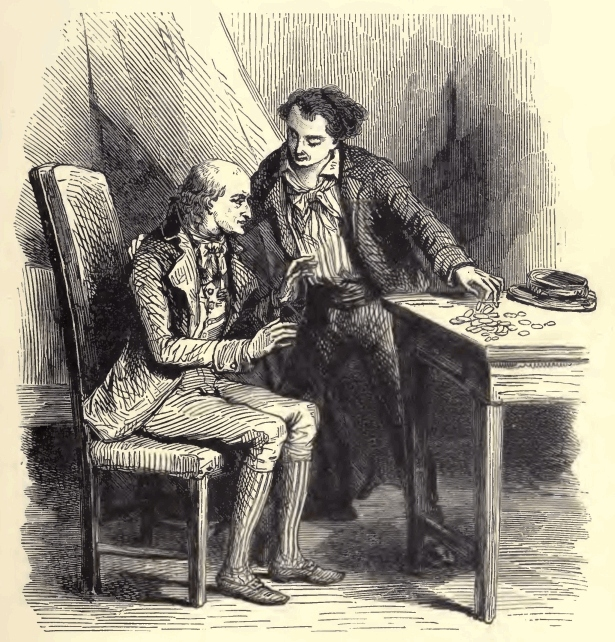
\includegraphics[width=\textwidth]{0035m.jpg}
\end{figure}

“Yes, here I am,” said the young man, “with a promising future and a
little money. Here, father, here!” he said, “take this—take it, and
send for something immediately.” And he emptied his pockets on the
table, the contents consisting of a dozen gold pieces, five or six
five-franc pieces, and some smaller coin. The countenance of old Dantès
brightened.

“Whom does this belong to?” he inquired.

“To me, to you, to us! Take it; buy some provisions; be happy, and
tomorrow we shall have more.”

“Gently, gently,” said the old man, with a smile; “and by your leave I
will use your purse moderately, for they would say, if they saw me buy
too many things at a time, that I had been obliged to await your
return, in order to be able to purchase them.”

“Do as you please; but, first of all, pray have a servant, father. I
will not have you left alone so long. I have some smuggled coffee and
most capital tobacco, in a small chest in the hold, which you shall
have tomorrow. But, hush, here comes somebody.”

“’Tis Caderousse, who has heard of your arrival, and no doubt comes to
congratulate you on your fortunate return.”

“Ah, lips that say one thing, while the heart thinks another,” murmured
Edmond. “But, never mind, he is a neighbor who has done us a service on
a time, so he’s welcome.”

As Edmond paused, the black and bearded head of Caderousse appeared at
the door. He was a man of twenty-five or six, and held a piece of
cloth, which, being a tailor, he was about to make into a coat-lining.

“What, is it you, Edmond, back again?” said he, with a broad
Marseillaise accent, and a grin that displayed his ivory-white teeth.

“Yes, as you see, neighbor Caderousse; and ready to be agreeable to you
in any and every way,” replied Dantès, but ill-concealing his coldness
under this cloak of civility.

“Thanks—thanks; but, fortunately, I do not want for anything; and it
chances that at times there are others who have need of me.” Dantès
made a gesture. “I do not allude to you, my boy. No!—no! I lent you
money, and you returned it; that’s like good neighbors, and we are
quits.”

“We are never quits with those who oblige us,” was Dantès’ reply; “for
when we do not owe them money, we owe them gratitude.”

“What’s the use of mentioning that? What is done is done. Let us talk
of your happy return, my boy. I had gone on the quay to match a piece
of mulberry cloth, when I met friend Danglars. ‘You at
Marseilles?’—‘Yes,’ says he.

“‘I thought you were at Smyrna.’—‘I was; but am now back again.’

“‘And where is the dear boy, our little Edmond?’

“‘Why, with his father, no doubt,’ replied Danglars. And so I came,”
added Caderousse, “as fast as I could to have the pleasure of shaking
hands with a friend.”

\begin{figure}[h]
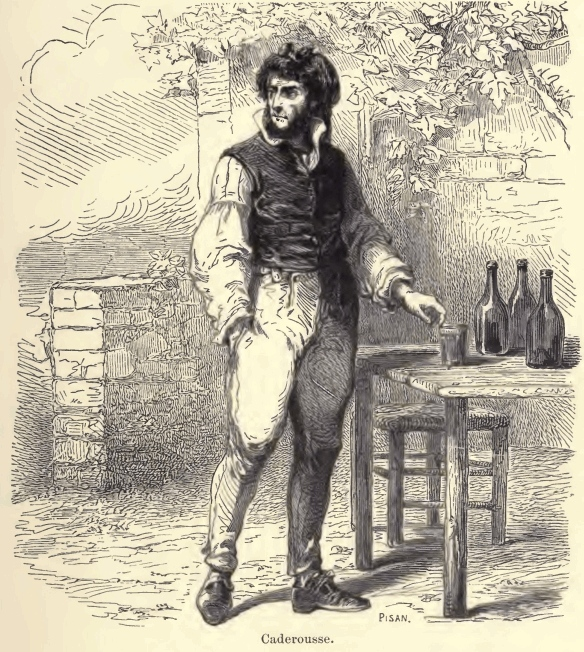
\includegraphics[width=\textwidth]{0037m.jpg}
\end{figure}

“Worthy Caderousse!” said the old man, “he is so much attached to us.”

“Yes, to be sure I am. I love and esteem you, because honest folks are
so rare. But it seems you have come back rich, my boy,” continued the
tailor, looking askance at the handful of gold and silver which Dantès
had thrown on the table.

The young man remarked the greedy glance which shone in the dark eyes
of his neighbor. “Eh,” he said, negligently, “this money is not mine. I
was expressing to my father my fears that he had wanted many things in
my absence, and to convince me he emptied his purse on the table. Come,
father” added Dantès, “put this money back in your box—unless neighbor
Caderousse wants anything, and in that case it is at his service.”

“No, my boy, no,” said Caderousse. “I am not in any want, thank God, my
living is suited to my means. Keep your money—keep it, I say;—one never
has too much;—but, at the same time, my boy, I am as much obliged by
your offer as if I took advantage of it.”

“It was offered with good will,” said Dantès.

“No doubt, my boy; no doubt. Well, you stand well with M. Morrel I
hear,—you insinuating dog, you!”

“M. Morrel has always been exceedingly kind to me,” replied Dantès.

“Then you were wrong to refuse to dine with him.”

“What, did you refuse to dine with him?” said old Dantès; “and did he
invite you to dine?”

“Yes, my dear father,” replied Edmond, smiling at his father’s
astonishment at the excessive honor paid to his son.

“And why did you refuse, my son?” inquired the old man.

“That I might the sooner see you again, my dear father,” replied the
young man. “I was most anxious to see you.”

“But it must have vexed M. Morrel, good, worthy man,” said Caderousse.
“And when you are looking forward to be captain, it was wrong to annoy
the owner.”

“But I explained to him the cause of my refusal,” replied Dantès, “and
I hope he fully understood it.”

“Yes, but to be captain one must do a little flattery to one’s
patrons.”

“I hope to be captain without that,” said Dantès.

“So much the better—so much the better! Nothing will give greater
pleasure to all your old friends; and I know one down there behind the
Saint Nicolas citadel who will not be sorry to hear it.”

“Mercédès?” said the old man.

“Yes, my dear father, and with your permission, now I have seen you,
and know you are well and have all you require, I will ask your consent
to go and pay a visit to the Catalans.”

“Go, my dear boy,” said old Dantès; “and Heaven bless you in your wife,
as it has blessed me in my son!”

“His wife!” said Caderousse; “why, how fast you go on, father Dantès;
she is not his wife yet, as it seems to me.”

“No, but according to all probability she soon will be,” replied
Edmond.

“Yes—yes,” said Caderousse; “but you were right to return as soon as
possible, my boy.”

“And why?”

“Because Mercédès is a very fine girl, and fine girls never lack
followers; she particularly has them by dozens.”

“Really?” answered Edmond, with a smile which had in it traces of
slight uneasiness.

\begin{figure}[h]
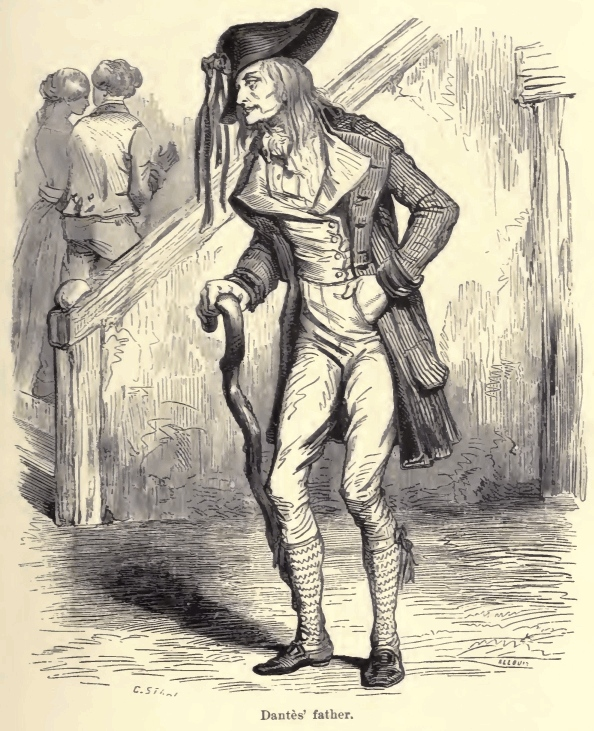
\includegraphics[width=\textwidth]{0039m.jpg}
\end{figure}

“Ah, yes,” continued Caderousse, “and capital offers, too; but you
know, you will be captain, and who could refuse you then?”

“Meaning to say,” replied Dantès, with a smile which but ill-concealed
his trouble, “that if I were not a captain——”

“Eh—eh!” said Caderousse, shaking his head.

“Come, come,” said the sailor, “I have a better opinion than you of
women in general, and of Mercédès in particular; and I am certain that,
captain or not, she will remain ever faithful to me.”

“So much the better—so much the better,” said Caderousse. “When one is
going to be married, there is nothing like implicit confidence; but
never mind that, my boy,—go and announce your arrival, and let her know
all your hopes and prospects.”

“I will go directly,” was Edmond’s reply; and, embracing his father,
and nodding to Caderousse, he left the apartment.

Caderousse lingered for a moment, then taking leave of old Dantès, he
went downstairs to rejoin Danglars, who awaited him at the corner of
the Rue Senac.

“Well,” said Danglars, “did you see him?”

“I have just left him,” answered Caderousse.

“Did he allude to his hope of being captain?”

“He spoke of it as a thing already decided.”

“Indeed!” said Danglars, “he is in too much hurry, it appears to me.”

“Why, it seems M. Morrel has promised him the thing.”

“So that he is quite elated about it?”

“Why, yes, he is actually insolent over the matter—has already offered
me his patronage, as if he were a grand personage, and proffered me a
loan of money, as though he were a banker.”

“Which you refused?”

“Most assuredly; although I might easily have accepted it, for it was I
who put into his hands the first silver he ever earned; but now M.
Dantès has no longer any occasion for assistance—he is about to become
a captain.”

“Pooh!” said Danglars, “he is not one yet.”

“\textit{Ma foi!} it will be as well if he is not,” answered Caderousse; “for
if he should be, there will be really no speaking to him.”

“If we choose,” replied Danglars, “he will remain what he is; and
perhaps become even less than he is.”

“What do you mean?”

“Nothing—I was speaking to myself. And is he still in love with the
Catalane?”

“Over head and ears; but, unless I am much mistaken, there will be a
storm in that quarter.”

\begin{figure}[h]
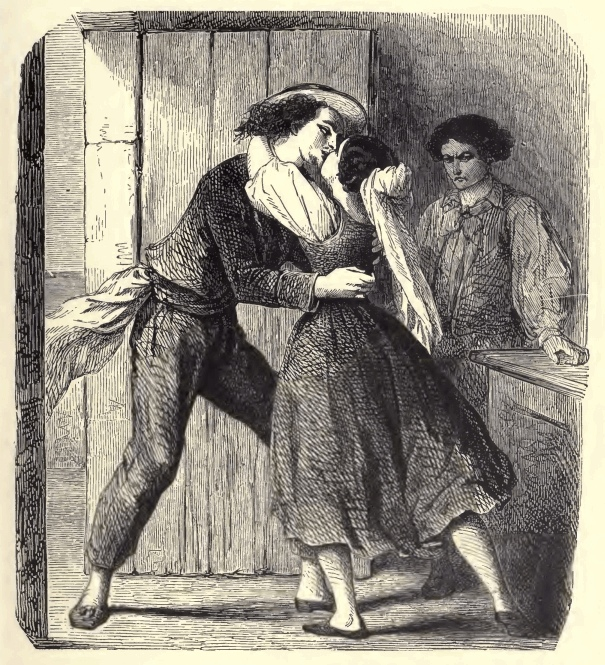
\includegraphics[width=\textwidth]{0041m.jpg}
\end{figure}

“Explain yourself.”

“Why should I?”

“It is more important than you think, perhaps. You do not like Dantès?”

“I never like upstarts.”

“Then tell me all you know about the Catalane.”

“I know nothing for certain; only I have seen things which induce me to
believe, as I told you, that the future captain will find some
annoyance in the vicinity of the Vieilles Infirmeries.”

“What have you seen?—come, tell me!”

“Well, every time I have seen Mercédès come into the city she has been
accompanied by a tall, strapping, black-eyed Catalan, with a red
complexion, brown skin, and fierce air, whom she calls cousin.”

“Really; and you think this cousin pays her attentions?”

“I only suppose so. What else can a strapping chap of twenty-one mean
with a fine wench of seventeen?”

“And you say that Dantès has gone to the Catalans?”

“He went before I came down.”

“Let us go the same way; we will stop at La Réserve, and we can drink a
glass of La Malgue, whilst we wait for news.”

“Come along,” said Caderousse; “but you pay the score.”

“Of course,” replied Danglars; and going quickly to the designated
place, they called for a bottle of wine, and two glasses.

Père Pamphile had seen Dantès pass not ten minutes before; and assured
that he was at the Catalans, they sat down under the budding foliage of
the planes and sycamores, in the branches of which the birds were
singing their welcome to one of the first days of spring.
